\newpage
\section{Setup} \label{sec:method}
\begin{itemize}
    \item laser beam diameter: 1.2mm +/- 0.5mm
    \item material length: 30cm
    \item triangle side length: 40cm
    \item tube diameter 3.5cm
\end{itemize}

\begin{figure}[h!]
    \centering
    \begin{tikzpicture}[scale=0.7]

    \draw[thick, rotate around={45:(0,17.2)}] (-1,17.2) rectangle (1,18.2);
    
    \draw[rotate around={60:(10,11.55)}] (9.5,11.55) rectangle (10.5,12.55);
    \draw[thick, rotate around={60:(10,11.55)}] (9.5,11.55) rectangle (10.5,11.45);
    \draw[rotate around={-210:(10,17.2)}] (9.5,17.2) rectangle (10.5,18.2);
    \draw[thick, rotate around={-210:(10,17.2)}] (9.5,17.2) rectangle (10.5,17.1);
    
    \draw[thick, rotate around={60:(7.5,12.9)}] (7,12.4) rectangle (8,13.4);
    \draw[thick, rotate around={60:(7.5,12.9)}] (7,12.4) to (8,13.4);
    \draw[thick, rotate around={60:(7.5,12.9)}] (8,12.4) to (7,13.4);

    \draw[thick, rotate around={120:(0,0)}] (-1,0) rectangle (1,1);
    \draw[thick, rotate around={240:(10,0)}] (9,0) rectangle (11,1);
    \draw[thick] (4,8.6) rectangle (6,9.6);

    \draw[red, thick] (2,0) to (0,0) to (5,8.6) to (10,0) to (8,0);
    \draw[red, photon] (2,0) to (8,0);
    \draw[rounded corners] (2,-0.5) rectangle (8,0.5);
    
    \draw[red, dashed] (0,0) to (10,17.2);
    \draw[red, dashed] (10,0) to (0,17.2);
    \draw[red, dashed] (10,11.55) to (0,17.2);
    
    
    \draw[green, dashed] (-3,0) to (0,0);
    \draw[] (-5,0.2) rectangle (-3,-0.2);
    
    \draw[] (5,3.7) circle (0.3);
    \filldraw[] (5,3.7) circle (0.1);
    \draw[thick,->] ([shift=(30:1cm)]5,3.7) arc (30:150:1cm);

    
    
    \node at (5,5.2) {$\Omega$};
    \node at (5,-1) {Resonator};
    \node at (-4,-0.7) {Guiding Laser};
    \node at (-1,1.5) {S1};
    \node at (11,1.5) {S2};
    \node at (3.3,9.1) {S3};
    \node at (-1,18.5) {S4};
    \node at (7,15) {Beam};
    \node at (7,14.5) {Splitter};
    \node at (10,10.2) {Photodiode};
    \node at (10,18.5) {Photodiode};
    
    \end{tikzpicture}
    \caption{Top view of the schematic setup of the experiment. The table rotates with angular velocity $\omega$ around the indicated axis.}
    \label{fig:setup}
\end{figure}


\begin{figure}[h!]
    \centering
    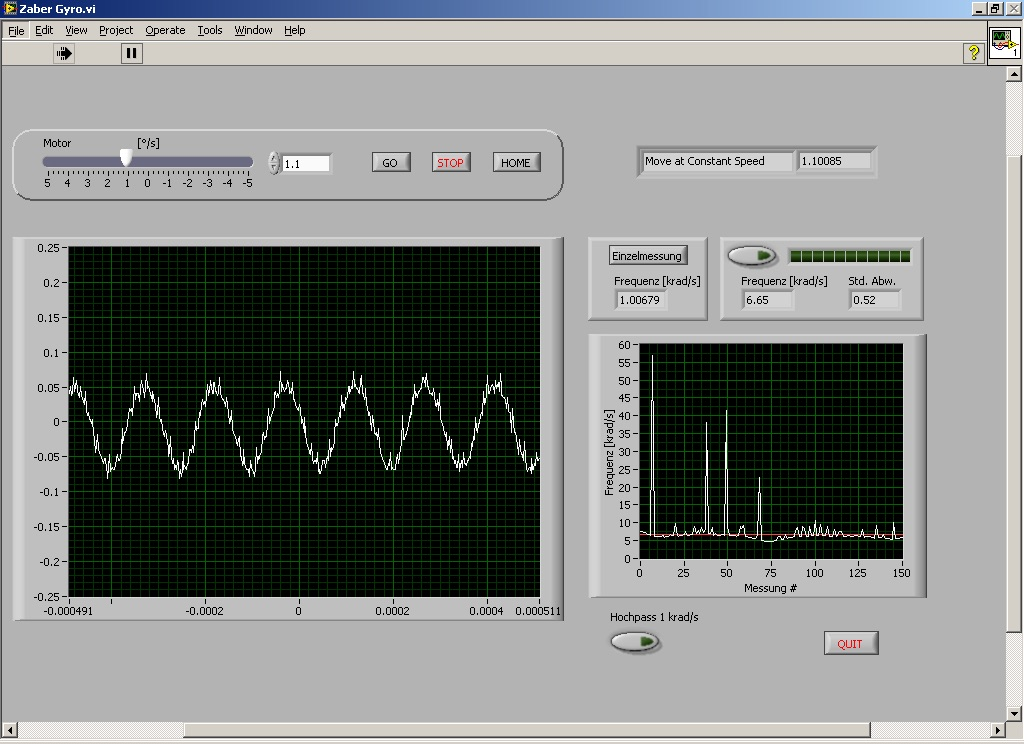
\includegraphics[width=\textwidth]{Gyroscope/Report/pictures/donatlinus.jpg}
    \caption{A screen shot of the Computer Interface in LabView during nominal operation.}
    \label{fig:screenshot}
\end{figure}

        
\begin{figure}[h!]
    \centering
    
\begin{tikzpicture}[scale=1]
        \foreach \i in {0.02,0.04,...,2.34}
        {
             \pgfmathsetmacro{\shade}{8.5 + 90*sin(\i*7*50)}
             \draw[thick,color=white!\shade!red] (0,0) circle (\i);
        }
    \end{tikzpicture}
    \caption{Interference pattern visible when the two beams are aligned.}
    \label{fig:interference}
\end{figure}